%\documentclass[10pt]{article}
%\usepackage{graphicx}
%\usepackage{amsmath}
%\usepackage{fullpage}
%\usepackage[icelandic]{babel}
%\usepackage[T1]{fontenc}
%\usepackage[utf8x]{inputenc}	
%
%\title{Forecasting Models}
%\author{David Erik Mollberg \and Guðjón Ingibergur Ólafsson \and Gunnar Gylfason \and Magnea Gunnarsdóttir \and Rebekka Jóhannsdóttir \and Róbert Árnason \and Steindór Tryggvason \and Styrmir Gauti Fjeldsted \and Vésteinn Sigurjónsson}
%
%\begin{document}
%\maketitle

\section {Sveiflur og letni(e.trends)}
 

Þegar spá þarf fyrir um sveiflur eða trend sem eru í gangi þá þarf að passa að velja réttar spár. Gagnlegt er að líta á vöxt fyrirtækinsins og markaðarins í sölu/aðgerðum, þegar litið er á gögn um mánaða eða árabil og augljóst mynstur er milli daga, vikna eða mánaða má áætla að mynstrið haldi áfram og hægt að yfirfara það í spá. 

\subsection{Figures}


\begin{figure}[htb]
\begin{center}

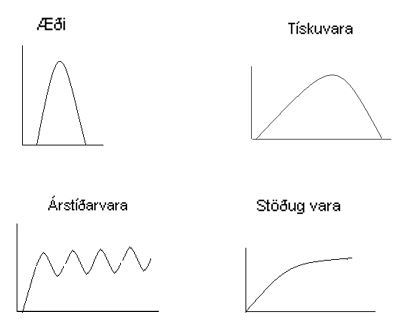
\includegraphics[width=0.75\textwidth]{tegundirspar}
\caption{Hérna sérst mismunandi eftirspurn sem þarf að spá fyrir}
\label{fig:figure1}
\end{center}
\end{figure}

\subsection{Aðferðir}
Árstíðarsveiflur eða vikusveiflu geta verið metna með árstíðarsveiflustðulum (e.seasonal index), getur verið háð eða óháð breytingu á meðal eftirspurnar.



	

\subsection{Jöfnur}

	$y =$ tímabilsgögn\\
	$I =$	árstíðar stuðull \\
	$L =$ fjöldi lotna á tímabili \\
	$A_p =$ meðaltal fyrir lotu á tímabili\\


	$$ I =  A_p/(y/L) $$\\


%\end{document}